\documentclass[10pt]{article}
\usepackage{amssymb,amsmath,times,url,graphicx,amsthm,alltt}
%\usepackage[pdftex,urlcolor=blue,pdfpagemode=none,pdfstartview=FitH]{hyperref}
\usepackage{my_packages}
\usepackage{tikz_packages}
%% url smaller font.
\makeatletter
\def\url@leostyle{%
  \@ifundefined{selectfont}{\def\UrlFont{\sf}}{\def\UrlFont{\small\ttfamily}}}
\makeatother
\urlstyle{leo}

%\usepackage[all,import]{xy}

\renewcommand{\baselinestretch}{1.2}
\date{}

\renewcommand{\thesubsection}{\arabic{subsection}. }
\renewcommand{\thesubsubsection}{\arabic{subsection}.\arabic{subsubsection} }

\theoremstyle{definition}
\newtheorem{prob}{Problem}[section]
%\renewcommand{\theprob}{\arabic{section}.\arabic{prob}}
\renewcommand{\theprob}{\arabic{prob}}

\newenvironment{subprob}%
{\renewcommand{\theenumi}{\alph{enumi}}\renewcommand{\labelenumi}{(\theenumi)}\begin{enumerate}}%
{\end{enumerate}}%

\newenvironment{matlab}
{\begin{alltt}\small\renewcommand{\baselinestretch}{1.2}\selectfont}%
{\end{alltt}}


\begin{document}

\pagestyle{empty}
\section*{MAE3145: Homework 2}
\vspace*{-0.4cm}
\noindent{Due date: \SI{2458022.197917}{\julianday}}%\\%\vspace*{0.5cm}

\begin{prob}
    The Juno spacecraft was launched August 5, 2011 and is now in orbit of Jupiter, having inserted into an highly elliptical Jovian orbit on July 5, 2016.
    Juno is the first deep-space vehicle to use solar panels at Jupiter, as all previous missions have relied on radioisotope thermoelectric generators. 
    Furthermore, considerable effort has been expended in the design of the orbit of Juno in the Jovian system. 
    Due to the extreme distance, the orbit is chosen to provide nearly continuous solar illumination, and to avoid the intense radiation environment of Jupiter.
    \begin{figure}[htbp]
        \centering
        \begin{subfigure}[htbp]{0.5\textwidth} 
            \includegraphics[height=5cm, keepaspectratio]{figures/juno.jpg} 
            \caption{Juno Spacecraft \label{fig:juno}} 
        \end{subfigure}\hfill
        \begin{subfigure}[htbp]{0.5\textwidth} 
            \includegraphics[height=5cm,keepaspectratio]{figures/trajectory.jpg} 
            \caption{Trajectory \label{fig:trajectory<`4`>}} 
        \end{subfigure} 
    \end{figure}
        
    After arriving in the Jovian system, Juno first entered a highly elliptical orbit which passed the orbit of the moon Callisto.
    Assume that during the first capture orbit the bodies are aligned as shown in~\cref{fig:planets}.
    \begin{figure}[htbp]
        \centering
        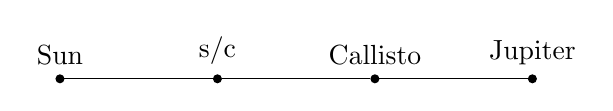
\begin{tikzpicture}
            [
            point/.style = {draw, circle, fill = black, inner sep = 1pt},
            dot/.style = {draw, circle, fill = black, inner sep = 0.2pt}
            ]
            % three corners of the triangle
            \node (s) at (0, 0) [point, label = {Sun}] {};
            \node (sc) at (2, 0) [point, label = {s/c}] {};
            \node (c) at (4, 0) [point, label = {Callisto}] {};
            \node (j) at (6, 0) [point, label = {Jupiter}] {};

            \draw (s) -- (sc) -- (c) -- (j);
        \end{tikzpicture}
        \caption{Planet alignment~\label{fig:planets}}
    \end{figure}
    
    Assume all bodies are in circular orbits with a radius equal to their semimajor axis. 
    A table of constants for some planetary moons has been provided on Blackboard.
    During orbit insertion, Juno passed within \textbf{\SI{4000}{\kilo\meter}} from the center of Callisto!

    \begin{subprob}
        \item At this instant, calculate the accelerations on the spacecraft with respect to Jupiter due to the gravity fields from the Sun, Callisto and Jupiter.
            Determine the dominant, direct, and indirect accelerations, including the directions. 

            Which one is the smallest? Largest? Is the dominant acceleration actually the largest?

        \item Determine the magnitude and direction of the perturbing accelerations. 
            Which body delivers the largest perturbing acceleration?
            For this alignment, consider each perturbing term. 
            Does the perturbing acceleration from the Sun tend to pull the spacecraft and Jupiter apart or drive the bodies together?
            What about the perturbation from Callisto?

        \item Given this four-body system, for the orbit of the spacecraft with respect to Jupiter, is a two-body orbit model sufficient to represent the path?
            If you had to decide to keep only one additional body in the model, would you keep the Sun or Callisto at this instant?
    \end{subprob}
    
    \begin{figure}[htbp]
        \centering
        \begin{subfigure}[htbp]{0.7\textwidth} 
            \includegraphics[width=\textwidth,keepaspectratio]{figures/jupiter_orbit.jpg} 
            \caption{ Jupiter Orbits} 
        \end{subfigure}

        \begin{subfigure}[htbp]{0.7\textwidth} 
            \includegraphics[width=\textwidth,keepaspectratio]{figures/jupiter_radiation.jpg} 
            \caption{Radiation at Jupiter} 
        \end{subfigure} 
        \caption{Juno orbits about Jupiter. The orbit plane is chosen to lie orthogonal to the Sun-Jupiter vector. In other words, the orbit angular momentum vector is designed such that it aligns with the direction to the Sun. This ensures that Juno is always illuminated and the polar orbits avoid the majority of the radiation environment at Jupiter.~\label{fig:jupiter_orbit}}
    \end{figure}
\end{prob}

\begin{prob}
    Consider the \underline{relative two-body} problem of the Earth and an orbiting spacecraft.
    An Earth-orbiting vehicle is tracked from ground stations: the spacecraft mass is \SI{500}{\kilo\gram}.
    At a certain instant, \( t_0 \), the following position and velocity are obtained relative to an inertial observer:
    \begin{itemize}
        \item Altitude is \SI{2000}{\kilo\meter} (remember that altitude above the Earth  \textbf{IS NOT} the same as distance from the Earth)
        \item Radial component of relative velocity is \SI{-1.2}{\kilo\meter\per\sec}
        \item Transverse component of relative velocity is \SI{6.7}{\kilo\meter\per\second}
    \end{itemize}

    Assume that our tracking system is perfect and these measurements are made without any error.
    \begin{subprob}
        \item Compute the total system angular momentum vector \( \bar C_3 \), specific angular momentum, total kinetic energy, total energy \( C_4 \), specific energy and area velocity.
        \item Within the context of the relative two-body problem, determine the following orbital characteristics: \( p, e, a, P, \theta^* \).
            Write the position vector in terms of the inertial unit vectors \( \hat e\) and \( \hat p \), or \( \hat p \) and \( \hat q \) (perifocal reference frame).
        \item Compare this relative velocity to the circular relative velocity at this altitude.
    \end{subprob}
\end{prob}

\clearpage
\newpage
\begin{prob}
    The Trojan asteroids are located at the vertex of an equilateral triangle with the Sun and Jupiter.
    \begin{figure}[htbp]
        \centering
        \subcaptionbox{Trojan Asteroids\label{fig:trojan_view}}{\includegraphics[width=0.5\textwidth,keepaspectratio]{figures/Trojans.jpg}}~
        \subcaptionbox{Trojan Asteroid schematic}{
        \begin{tikzpicture}
            [
            point/.style = {draw, circle, fill = black, inner sep = 1pt},
            dot/.style = {draw, circle, fill = black, inner sep = 0.2pt}
            ]
            % three corners of the triangle
            \node (s) at (0, 0) [point, label = {below:Sun}] {};
            \node (ast) at (3, 5) [point, label = {Trojan Asteroid}] {};
            \node (j) at (6, 0) [point, label = {below:Jupiter}] {};

            \draw (s) -- (ast) node[pos=0.5, above left] {\(R\)}; 
            \draw (ast) -- (j) node[pos=0.5, above right] {\(R\)}; 
            \draw (j) -- (s) node[pos=0.5,below] {\(R\)};
        \end{tikzpicture}
        }
    \end{figure}

    \begin{subprob}
        \item Write an expression for the acceleration of a Trojan asteroid relative to the sun. 
            Determine the dominant and the net perturbing accelerations.
            Compare them in terms of both magnitude and directions.
            Does Jupiter act to drive the asteroid closer to the Sun or further away.
            Do you think the influence of the sun or Jupiter is more significant?
            Why?
        \item Reformulate the problem to determine the acceleration of a Trojan asteroid relative to Jupiter.
            Now compute the dominant and the net perturbing accelerations. 
            Does the sun drive the asteroid closer to Jupiter or away from the planet?
            Is the Sun or Jupiter more significant?
        \item Which of the two formulations is correct?
            Why?
    \end{subprob}
\end{prob}
\end{document}

